\documentclass[11pt,a4paper]{article}
% Shared preamble for CYS 4151 lab reports (network config + execution guide)
\NeedsTeXFormat{LaTeX2e}

\usepackage[margin=2.2cm,headheight=28pt]{geometry}
\usepackage[table,xcdraw]{xcolor}
\usepackage{fontspec}

% force the PDF's copy/search text layer to record the exact original input
% characters (ActualText), not whatever codepoint xdvipdfmx's font-cmap
% heuristic would otherwise pick for a shared glyph (this is what was turning
% a typed ASCII hyphen-minus "-" into a copy-pasted Unicode hyphen "‐" U+2010,
% silently breaking every copy-pasted shell command that uses a "-flag")
\XeTeXgenerateactualtext=1

\setmainfont{Calibri}[
  BoldFont = Calibri Bold,
  ItalicFont = Calibri Italic,
  BoldItalicFont = Calibri Bold Italic
]
\setmonofont{Consolas}

\usepackage{booktabs}
\usepackage{array}
\usepackage{longtable}
\usepackage{tabularx}
\usepackage{graphicx}
\usepackage{tikz}
\usetikzlibrary{shapes.geometric,arrows.meta,positioning,fit,backgrounds,calc}
\usepackage[most]{tcolorbox}
\usepackage{enumitem}
\usepackage{fancyhdr}
\usepackage[hypcap=false]{caption}
\usepackage{titlesec}
\usepackage{hyperref}
\usepackage{pifont}
\usepackage{multirow}
\usepackage{rotating}
\usepackage{lastpage}
\usepackage{fancyvrb}
\usepackage{needspace}

\providecommand{\DocShortTitle}{}

% ---------- colour palette ----------
\definecolor{navy}{HTML}{1B2A4A}
\definecolor{steel}{HTML}{2E5C8A}
\definecolor{blueteam}{HTML}{1F6FB2}
\definecolor{blueteamlight}{HTML}{DCEBF7}
\definecolor{redteam}{HTML}{B23A2E}
\definecolor{redteamlight}{HTML}{FBE2DF}
\definecolor{targetgrey}{HTML}{5A5A5A}
\definecolor{targetlight}{HTML}{E9E9E9}
\definecolor{accentgold}{HTML}{C8922A}
\definecolor{lightgrey}{HTML}{F4F6F8}
\definecolor{codebg}{HTML}{F7F7F9}
\definecolor{codeborder}{HTML}{C9CDD3}
\definecolor{okgreen}{HTML}{2E7D32}
\definecolor{warnamber}{HTML}{B8860B}

% ---------- column helpers ----------
\newcolumntype{L}[1]{>{\raggedright\arraybackslash}p{#1}}
\newcolumntype{C}[1]{>{\centering\arraybackslash}p{#1}}

% ---------- headings ----------
\titleformat{\section}{\large\bfseries\color{navy}}{\thesection}{0.6em}{}[{\color{steel}\titlerule[0.8pt]}]
\titleformat{\subsection}{\normalsize\bfseries\color{steel}}{\thesubsection}{0.6em}{}
\titleformat{\subsubsection}{\normalsize\bfseries\color{navy}}{\thesubsubsection}{0.6em}{}

\pagestyle{fancy}
\fancyhf{}
\renewcommand{\headrulewidth}{0.6pt}
\renewcommand{\footrulewidth}{0.4pt}
\lhead{\small\color{navy}\textbf{CYS 4151 -- Ethical Hacking Lab}}
\rhead{\small\color{navy}\DocShortTitle}
\lfoot{\small\color{targetgrey}SecureTech Solutions Ltd. Security Assessment}
\rfoot{\small\color{targetgrey}Page \thepage\ of \pageref{LastPage}}

\hypersetup{
  colorlinks=true,
  linkcolor=steel,
  citecolor=steel,
  urlcolor=steel,
  pdfborder={0 0 0}
}

% ---------- command/comment boxes ----------
\newtcolorbox{cmdbox}[1][]{
  enhanced, breakable, colback=codebg, colframe=codeborder, boxrule=0.5pt,
  arc=2pt, left=6pt, right=6pt, top=4pt, bottom=4pt,
  fonttitle=\bfseries\small, coltitle=navy,
  title={#1}
}

\newtcolorbox{expectbox}{
  enhanced, breakable, colback=blueteamlight!60, colframe=blueteam, boxrule=0.5pt,
  arc=2pt, left=6pt, right=6pt, top=3pt, bottom=3pt,
  fonttitle=\bfseries\small, coltitle=white, colbacktitle=blueteam,
  title={Expected Outcome}
}

\newtcolorbox{troublebox}{
  enhanced, breakable, colback=redteamlight!50, colframe=redteam, boxrule=0.5pt,
  arc=2pt, left=6pt, right=6pt, top=3pt, bottom=3pt,
  fonttitle=\bfseries\small, coltitle=white, colbacktitle=redteam,
  title={Difficulty Encountered}
}

\newtcolorbox{notebox}[1][Note]{
  enhanced, breakable, colback=lightgrey, colframe=accentgold, boxrule=0.5pt,
  arc=2pt, left=6pt, right=6pt, top=3pt, bottom=3pt,
  fonttitle=\bfseries\small, coltitle=white, colbacktitle=accentgold,
  title={#1}
}

\newtcolorbox{redbox}[1][Red Team Strategy]{
  enhanced, breakable, colback=redteamlight!40, colframe=redteam, boxrule=0.7pt,
  arc=2pt, left=6pt, right=6pt, top=3pt, bottom=3pt,
  fonttitle=\bfseries\small, coltitle=white, colbacktitle=redteam,
  title={#1}
}

\newtcolorbox{bluebox}[1][Blue Team Strategy]{
  enhanced, breakable, colback=blueteamlight!50, colframe=blueteam, boxrule=0.7pt,
  arc=2pt, left=6pt, right=6pt, top=3pt, bottom=3pt,
  fonttitle=\bfseries\small, coltitle=white, colbacktitle=blueteam,
  title={#1}
}

% ---------- nickname badges ----------
\newcommand{\pcbadge}[2]{%
  \tikz[baseline=-0.6ex]\node[rectangle,rounded corners=2pt,inner sep=3pt,
    fill=#1!85!black,text=white,font=\scriptsize\bfseries]{#2};%
}
\newcommand{\marshall}{\pcbadge{blueteam}{PC1 Marshall}}
\newcommand{\fahdil}{\pcbadge{blueteam}{PC2 Fahdil}}
\newcommand{\rayan}{\pcbadge{redteam}{PC3 Rayan}}
\newcommand{\bruno}{\pcbadge{redteam}{PC4 Bruno}}
\newcommand{\amina}{\pcbadge{blueteam}{PC5 Amina}}

\newcommand{\thd}[1]{\textcolor{white}{\textbf{#1}}}

% ---------- verbatim command blocks (safe for #, $, %, &, ^, _, ~, {, }, \) ----------
\DefineVerbatimEnvironment{cmdverb}{Verbatim}{fontsize=\small}

\newlist{steps}{enumerate}{2}
\setlist[steps]{label=\arabic*., left=1.2em, itemsep=2pt, topsep=3pt}

\AtBeginDocument{\renewcommand{\arraystretch}{1.25}}

\renewcommand{\DocShortTitle}{Lab Network Configuration}

\title{\color{navy}\textbf{CYS 4151 --- Ethical Hacking Lab}\\[4pt]
\Large Network Configuration \& Build Guide}
\author{}
\date{}

\begin{document}
\pagenumbering{gobble}

% ===================== TITLE PAGE =====================
\begin{titlepage}
\centering
\vspace*{1.2cm}
{\Huge\bfseries\color{navy} CYS 4151 Ethical Hacking Lab}\\[10pt]
{\Large\color{steel} Network Configuration \& Build Guide}\\[4pt]
{\large\color{targetgrey} SecureTech Solutions Ltd. --- Enterprise Security Assessment}\\[28pt]

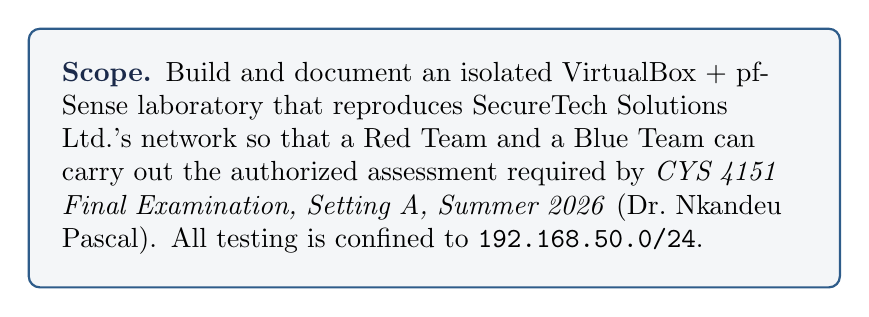
\begin{tikzpicture}
\node[rectangle,rounded corners=4pt,draw=steel,line width=0.8pt,fill=lightgrey,
  inner sep=12pt,text width=0.78\textwidth] {
  \raggedright
  \textbf{\color{navy}Scope.} Build and document an isolated VirtualBox + pfSense
  laboratory that reproduces SecureTech Solutions Ltd.'s network so that a Red Team
  and a Blue Team can carry out the authorized assessment required by
  \emph{CYS 4151 Final Examination, Setting A, Summer 2026} (Dr.\ Nkandeu Pascal).
  All testing is confined to \texttt{192.168.50.0/24}.
};
\end{tikzpicture}

\vspace{28pt}
{\large\bfseries\color{navy} Lab Team}\\[10pt]
\renewcommand{\arraystretch}{1.5}
\begin{tabular}{c c c c}
\marshall & \fahdil & \rayan & \bruno \\
\end{tabular}

\vspace{6pt}
\begin{tabular}{c}
\amina
\end{tabular}

\vfill
{\color{targetgrey}\small Course: CYS 4151 Ethical Hacking \quad|\quad Venue: Cisco Lab \quad|\quad Summer 2026}\\[4pt]
{\color{targetgrey}\small Document 1 of 2 --- see also \emph{CYS4151 Post-Configuration Execution Guide}}
\end{titlepage}

\pagenumbering{arabic}
\setcounter{page}{1}
\tableofcontents
\clearpage

% ===================== 1. INTRODUCTION =====================
\section{Introduction \& Scenario Recap}

SecureTech Solutions Ltd. is a 120-employee software and digital services company that
reported unauthorized login attempts, weak/reused passwords, suspicious web server
activity, possible customer data exposure, unpatched systems, and no centralized
monitoring. Our team was authorized, in writing, to simulate both a \textbf{Red Team}
(offensive) and a \textbf{Blue Team} (defensive) inside a contained laboratory only ---
never against production systems.

This document covers \textbf{Task 1 (Laboratory Design \& Documentation)}: the physical
and virtual network we built, every VM from first install to a verified static IP, the
real problems we hit while bringing the network up, and the pfSense access-control
configuration that enforces the lab's security boundary. The companion
\emph{Post-Configuration Execution Guide} picks up from here and walks Tasks 2--13.

\begin{notebox}[Authorized Scope]
All offensive and defensive activity described in both documents is confined to the
isolated lab segment \texttt{192.168.50.0/24}. Nothing here is ever pointed at a host
outside this range.
\end{notebox}

% ===================== 2. TEAM & ROLE ASSIGNMENT =====================
\section{Team \& Role Assignment}

Five physical host machines were used, one per student, each running one or more
VirtualBox guest VMs. Team colour follows the badge used throughout both documents.

\begin{center}
\renewcommand{\arraystretch}{1.4}
\begin{tabular}{l l l L{6.6cm}}
\toprule
\rowcolor{navy}
\thd{PC} & \thd{Team} & \thd{Lab IP(s)} & \thd{Primary Responsibility} \\
\midrule
\marshall & Blue & 192.168.50.1 & pfSense firewall/router (gateway for the whole lab) + a Kali VM running Suricata as an inline-monitoring IDS sensor. \\
\fahdil & Blue & 192.168.50.10 & Windows 10 workstation representing the ``employee computer'' asset; Blue Team hardens and audits it (password policy, patching). \\
\rayan & Red* & 192.168.50.20 (+.30, +.40 nested) & Builds and hosts the shared Server + DVWA/Juice Shop + Metasploitable2/3 targets; once the network is live, operates as Red Team against the wider lab. \\
\bruno & Red & 192.168.50.100 & Kali Linux --- primary offensive attack platform (recon, enumeration, exploitation). \\
\amina & Blue & 192.168.50.250 & OpenVAS/Greenbone vulnerability scanner --- automated assessment and CVSS triage. \\
\bottomrule
\end{tabular}
\end{center}

\footnotesize{*Rayan configures PC3 as shared infrastructure during the build phase
(Section~\ref{sec:pc3}); once connectivity is verified he switches hats and works
exclusively as a Red Team member for Tasks 2 onward.}
\normalsize

% ===================== 3. TOPOLOGY DIAGRAM =====================
\section{Network Topology}
\label{sec:topology}
\needspace{11cm}

\begin{figure}[ht]
\centering
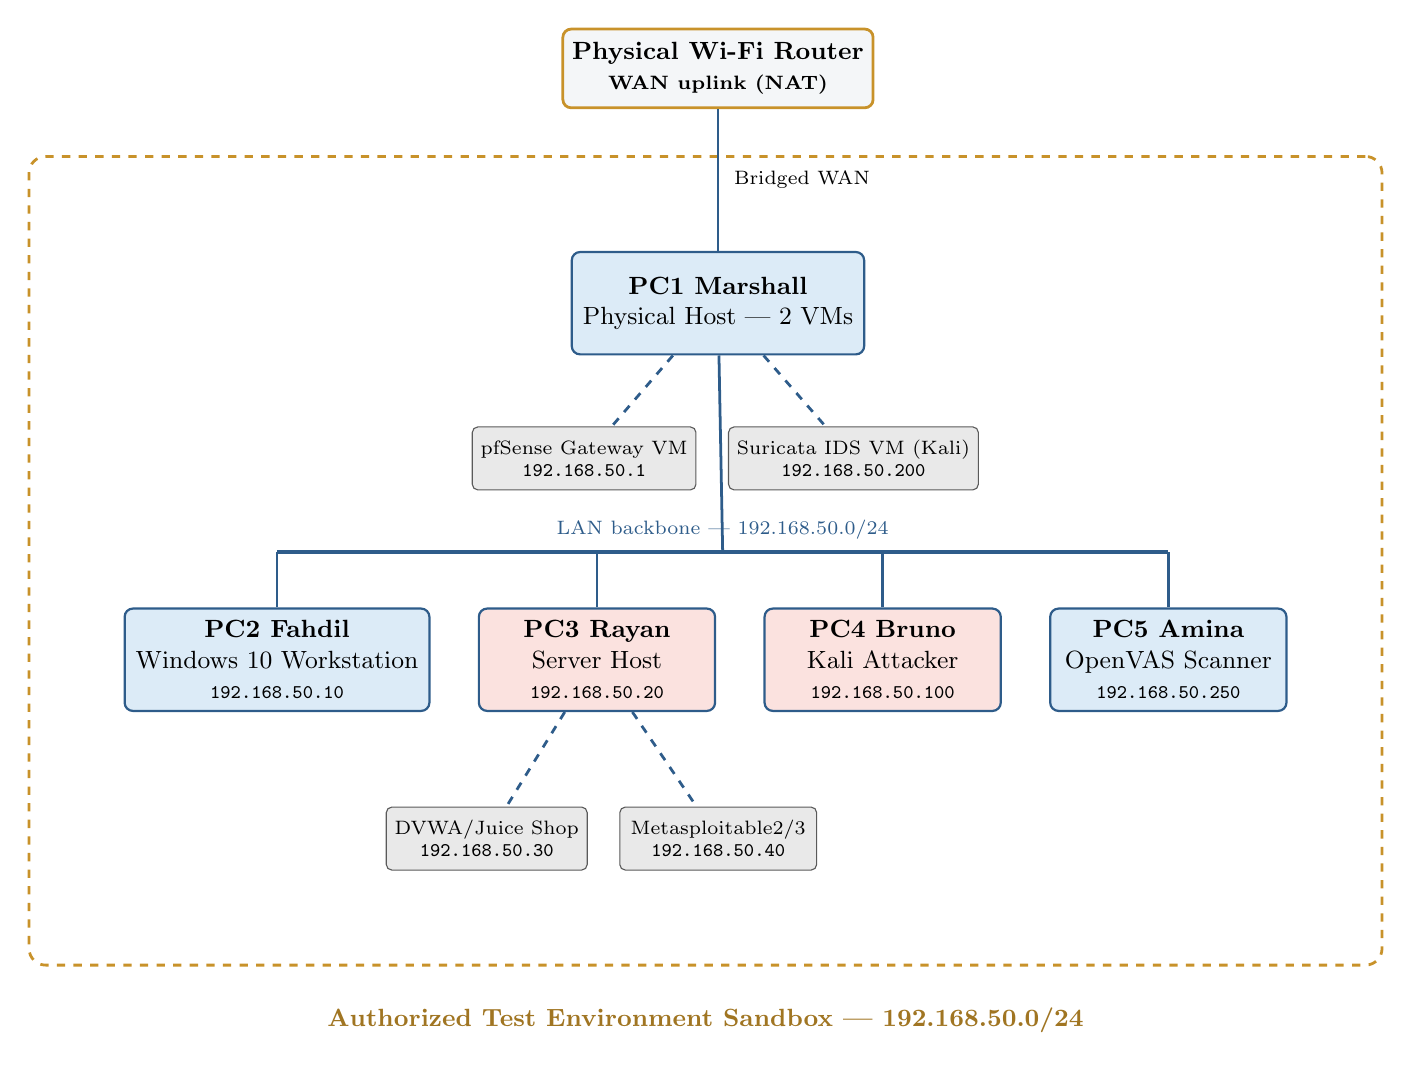
\begin{tikzpicture}[
  node distance=16mm and 7mm,
  pcbox/.style={rectangle, rounded corners=3pt, draw=steel, line width=0.8pt,
    minimum width=3.0cm, minimum height=1.3cm, align=center, font=\small, inner sep=4pt},
  bluepc/.style={pcbox, fill=blueteamlight},
  redpc/.style={pcbox, fill=redteamlight},
  nestedbox/.style={rectangle, rounded corners=2pt, draw=targetgrey, fill=targetlight,
    minimum width=2.5cm, minimum height=0.8cm, align=center, font=\scriptsize, inner sep=3pt},
  router/.style={rectangle, rounded corners=3pt, draw=accentgold, line width=1pt,
    fill=lightgrey, minimum width=3.2cm, minimum height=1.0cm, align=center, font=\small\bfseries},
  lanline/.style={line width=1pt, draw=steel}
]

% Physical Wi-Fi router (uplink only, outside the authorized sandbox)
\node[router] (wifi) {Physical Wi-Fi Router\\\scriptsize WAN uplink (NAT)};

% PC1 physical host runs two guest VMs: pfSense gateway + Suricata IDS (Kali)
\node[bluepc, below=18mm of wifi] (pc1) {\textbf{PC1 Marshall}\\Physical Host --- 2 VMs};
\draw[lanline] (wifi) -- (pc1) node[midway, right, font=\scriptsize, xshift=2pt]{Bridged WAN};

\node[nestedbox, below=9mm of pc1, xshift=-1.7cm] (pfsense) {pfSense Gateway VM\\\texttt{\scriptsize 192.168.50.1}};
\node[nestedbox, right=4mm of pfsense] (suricata) {Suricata IDS VM (Kali)\\\texttt{\scriptsize 192.168.50.200}};
\draw[lanline, dashed] (pc1) -- (pfsense);
\draw[lanline, dashed] (pc1) -- (suricata);

% Client PCs along the LAN backbone
\node[bluepc, below=32mm of pc1, xshift=-5.6cm] (pc2) {\textbf{PC2 Fahdil}\\Windows 10 Workstation\\\texttt{\scriptsize 192.168.50.10}};
\node[redpc,  right=6mm of pc2] (pc3) {\textbf{PC3 Rayan}\\Server Host\\\texttt{\scriptsize 192.168.50.20}};
\node[redpc,  right=6mm of pc3] (pc4) {\textbf{PC4 Bruno}\\Kali Attacker\\\texttt{\scriptsize 192.168.50.100}};
\node[bluepc, right=6mm of pc4] (pc5) {\textbf{PC5 Amina}\\OpenVAS Scanner\\\texttt{\scriptsize 192.168.50.250}};

% LAN backbone line, drawn between PC1 and the client row, clear of both
\coordinate (backboneL) at ($(pc2.north)+(0,7mm)$);
\coordinate (backboneR) at ($(pc5.north)+(0,7mm)$);
\draw[lanline, line width=1.4pt] (backboneL) -- (backboneR) coordinate[midway] (backbonemid);
\node[font=\scriptsize\color{steel}, above=1pt of backbonemid] {LAN backbone --- 192.168.50.0/24};
\draw[lanline] (pc1) -- (backbonemid);
\draw[lanline] (pc2.north) -- ($(pc2.north)+(0,7mm)$);
\draw[lanline] (pc3.north) -- ($(pc3.north)+(0,7mm)$);
\draw[lanline] (pc4.north) -- ($(pc4.north)+(0,7mm)$);
\draw[lanline] (pc5.north) -- ($(pc5.north)+(0,7mm)$);

% Nested targets under PC3
\node[nestedbox, below=12mm of pc3, xshift=-1.4cm] (dvwa) {DVWA/Juice Shop\\\texttt{\scriptsize 192.168.50.30}};
\node[nestedbox, right=4mm of dvwa] (msf) {Metasploitable2/3\\\texttt{\scriptsize 192.168.50.40}};
\draw[lanline, dashed] (pc3) -- (dvwa);
\draw[lanline, dashed] (pc3) -- (msf);

% Sandbox boundary: everything authorized for testing, router excluded
\begin{scope}[on background layer]
\node[draw=accentgold, dashed, line width=1pt, rounded corners=6pt,
  fit=(pc1)(pfsense)(suricata)(pc2)(pc3)(pc4)(pc5)(dvwa)(msf), inner sep=12mm] (sandbox) {};
\end{scope}
\node[below=4mm of sandbox, font=\small\bfseries, color=accentgold!80!black,
  align=center, text width=12cm] {Authorized Test Environment Sandbox --- 192.168.50.0/24};

\end{tikzpicture}

\vspace{5mm}
\resizebox{\textwidth}{!}{%

\begin{tikzpicture}[node distance=2mm]
\node[rectangle, draw=blueteam, fill=blueteamlight, minimum width=0.4cm, minimum height=0.4cm] (lg1) {};
\node[right=2pt of lg1, font=\scriptsize] (lg1t) {Blue Team (Defense)};
\node[rectangle, draw=redteam, fill=redteamlight, minimum width=0.4cm, minimum height=0.4cm, right=16mm of lg1t] (lg2) {};
\node[right=2pt of lg2, font=\scriptsize] (lg2t) {Red Team (Offense)};
\node[rectangle, draw=targetgrey, fill=targetlight, minimum width=0.4cm, minimum height=0.4cm, right=16mm of lg2t] (lg3) {};
\node[right=2pt of lg3, font=\scriptsize] (lg3t) {Vulnerable/Nested Target VM};
\node[rectangle, draw=accentgold, fill=lightgrey, minimum width=0.4cm, minimum height=0.4cm, right=16mm of lg3t] (lg4) {};
\node[right=2pt of lg4, font=\scriptsize] (lg4t) {External/Physical Infrastructure};
\end{tikzpicture}%
}

\caption{Corrected lab topology: PC1 (Marshall) and PC5 (Amina) anchor the Blue Team
defensive stack (firewall, IDS, and vulnerability scanning); PC2 (Fahdil) is the Blue
Team's hardened workstation asset; PC3 (Rayan) hosts the shared vulnerable targets and
transitions to Red Team once the network goes live; PC4 (Bruno) is the Red Team's
primary attack platform.}
\label{fig:topology}
\end{figure}

% ===================== 4. DESIGN STRATEGY =====================
\section{Design-Level Strategy}

\begin{redbox}[Red Team --- Network-Level Intent]
Rayan and Bruno treat \texttt{192.168.50.0/24} as the target range. Their plan is to
(1) sweep the whole subnet from Bruno's Kali box (PC4) to build an asset map, (2)
fingerprint the server/web/target stack hosted on Rayan's PC3, (3) look for a foothold
on the Metasploitable/DVWA targets first since they are intentionally weak, then (4)
pivot from that foothold toward Fahdil's workstation (PC2) to simulate lateral movement
toward an ``employee'' asset, all while assuming pfSense (PC1) and the OpenVAS/Suricata
nodes are watching --- i.e. they expect to be logged and plan noise-reduction (timing,
targeted scans) accordingly.
\end{redbox}

\begin{bluebox}[Blue Team --- Network-Level Intent]
Marshall, Fahdil and Amina assume the Red Team will enter through the weakest
advertised services (the DVWA/Metasploitable targets on PC3). Their plan is to (1) make
pfSense (PC1) the single chokepoint all inter-host traffic must cross, with a
default-deny LAN ruleset and only the narrow exceptions defined in
Section~\ref{sec:acl}; (2) run Suricata in the Kali VM on PC1 in promiscuous IDS mode
against the LAN backbone so every host-to-host flow is visible for detection, not just
WAN traffic; (3) run OpenVAS from PC5 proactively against the server/target stack so
known vulnerabilities are documented \emph{before} Red Team confirms them by exploiting
them; and (4) keep Fahdil's workstation (PC2) patched and its credential policy audited
so it is not the easy pivot target Red Team is hoping for.
\end{bluebox}

\clearpage

% ===================== 5. PC1 SETUP =====================
\section{PC1 --- Marshall: pfSense Gateway + Suricata IDS (Blue Team)}
\label{sec:pc1}

PC1 is the centralized firewall, router and traffic-inspection point for the entire
lab. It runs \emph{two} guest VMs under one VirtualBox hypervisor: a pfSense VM (LAN
gateway/firewall) and a Kali Linux VM dedicated to running Suricata as a passive IDS
sensor.

\subsection{Install VirtualBox and create the pfSense VM}
\begin{steps}
\item Install Oracle VirtualBox (and the matching Extension Pack) on the PC1 host machine.
\item Download the current pfSense CE installer ISO from the official pfSense site.
\item In VirtualBox: \textbf{New} $\to$ Name \texttt{pfSense-GW}, Type \texttt{BSD},
  Version \texttt{FreeBSD (64-bit)}.
\item Allocate \textbf{2048 MB RAM}, \textbf{2 vCPUs}, and a \textbf{20 GB} dynamically
  allocated VDI disk (pfSense itself is light; this leaves headroom for packages and logs).
\item Settings $\to$ Storage: attach the pfSense ISO to the virtual optical drive.
\item Settings $\to$ System $\to$ Processor: enable \textbf{PAE/NX}.
\end{steps}

\subsection{Network adapters for pfSense}
pfSense needs two NICs: one for the uplink (WAN) and one for the lab LAN.
\begin{steps}
\item Settings $\to$ Network $\to$ \textbf{Adapter 1 (WAN)}: Attached to
  \textbf{NAT}. This lets pfSense reach the internet (package/plugin downloads,
  patches) without exposing the lab.
\item Settings $\to$ Network $\to$ \textbf{Adapter 2 (LAN)}: Attached to
  \textbf{Bridged Adapter}, Name = the physical host's active Wi-Fi adapter. Expand
  \textbf{Advanced} and set \textbf{Promiscuous Mode: Allow All}.
\end{steps}

\begin{troublebox}[Host-Only Adapter attempt failed]
Our first attempt used a \textbf{Host-Only Adapter} for the LAN leg on every PC,
assuming it would behave like a normal lab switch. It did not work: a VirtualBox
Host-Only network is a virtual switch that exists \emph{only inside one physical
hypervisor} --- it never leaves that physical machine's NIC. Because our five students
are on five separate physical PCs connected only over Wi-Fi, each PC's VMs ended up on
their own isolated Host-Only segment with no path to the other four PCs: pings between
VMs on different physical machines timed out, DHCP requests to pfSense never arrived,
and pfSense's LAN interface only ever saw its own host's loopback traffic.
\textbf{Fix:} switch every LAN-side adapter (pfSense and all four clients) to
\textbf{Bridged Adapter} bound to each machine's physical Wi-Fi NIC, with
\textbf{Promiscuous Mode: Allow All}. Bridging makes every VM appear as its own device
directly on the physical Wi-Fi segment, so all five physical PCs' VMs can finally see
one another.
\end{troublebox}

\subsection{Initial pfSense console staging}
\begin{steps}
\item Power on the pfSense VM and let the installer finish; reboot into the console menu.
\item At the console menu, choose \textbf{2) Set interface IP address}.
\item Select the LAN interface, assign the static address \texttt{192.168.50.1}.
\item Enter the subnet bitmask: \texttt{24}.
\item When prompted, enable the DHCP server on LAN (optional --- we assign static
  addresses to every client instead, see Sections~\ref{sec:pc2}--\ref{sec:pc5}).
\end{steps}

\begin{expectbox}
The console menu reports the LAN interface as \texttt{192.168.50.1/24}, \texttt{UP}.
From any host already bridged onto the LAN segment:
\begin{cmdverb}
# confirm the gateway answers on the lab subnet
ping -c 4 192.168.50.1
\end{cmdverb}
returns 4 replies with low, stable latency.
\end{expectbox}

\subsection{pfSense web GUI initial setup wizard}
\begin{steps}
\item From a bridged client, browse to \texttt{https://192.168.50.1} and accept the
  self-signed certificate warning.
\item Log in with the default credentials (\texttt{admin} / \texttt{pfsense}) and
  immediately change the admin password under the setup wizard.
\item Set the hostname (\texttt{pfsense-gw}), domain, and DNS servers.
\item Confirm the WAN interface shows an address obtained via NAT/DHCP from the
  VirtualBox NAT engine, and the LAN interface shows \texttt{192.168.50.1/24}.
\item Finish the wizard and reload the GUI.
\end{steps}

\subsection{Suricata-in-Kali IDS VM (second VM on PC1)}
A second guest VM on the same PC1 hypervisor runs Kali Linux purely as a Suricata
sensor --- it is never used to attack, only to listen.

\begin{steps}
\item VirtualBox \textbf{New} $\to$ Name \texttt{PC1-Suricata-IDS}, Type \texttt{Linux},
  Version \texttt{Debian (64-bit)}. Allocate 4096 MB RAM, 2 vCPUs, 40 GB disk.
\item Attach the Kali Linux installer ISO and complete a standard installation.
\item Settings $\to$ Network $\to$ Adapter 1: \textbf{Bridged Adapter} on the same
  physical Wi-Fi NIC, \textbf{Promiscuous Mode: Allow All} (required so this VM can
  passively see LAN traffic that is not addressed to it).
\item Assign it a static management address, \texttt{192.168.50.200/24}, gateway
  \texttt{192.168.50.1}.
\end{steps}

\begin{cmdbox}[Suricata installation \& IDS mode]
\begin{cmdverb}
# update package lists and install Suricata
sudo apt update && sudo apt install -y suricata jq

# confirm the interface that should see LAN traffic
ip -brief addr show

# point Suricata at the lab subnet (HOME_NET)
sudo sed -i 's/^HOME_NET.*/HOME_NET: "[192.168.50.0\/24]"/' \
    /etc/suricata/suricata.yaml

# enable and start Suricata in IDS (listen-only) mode on the bridged interface
sudo systemctl enable --now suricata

# tail live alerts as JSON, filtered to readable fields
sudo tail -f /var/log/suricata/eve.json | jq 'select(.event_type=="alert")'
\end{cmdverb}
\end{cmdbox}

\begin{expectbox}
\texttt{systemctl status suricata} reports \texttt{active (running)}. The
\texttt{eve.json} tail stays idle until traffic matching a signature crosses the
bridged interface; once Red Team traffic starts in the companion Execution Guide, alert
JSON objects appear here in real time --- this is the evidence base for
Task 11 (Blue Team Investigation).
\end{expectbox}

\begin{notebox}[Why a Kali VM for Suricata instead of pfSense's own package]
pfSense ships a Suricata package that can run inline on its own interfaces, but we
deliberately run Suricata on a separate Kali VM in \emph{promiscuous, out-of-band} mode
instead. This keeps the firewall VM (PC1's pfSense guest) lean and dedicated purely to
routing/filtering, while the IDS sensor can be rebuilt, tuned, or have its ruleset
updated without any risk of taking down the lab's only gateway.
\end{notebox}

\clearpage

% ===================== 6. PC2 SETUP =====================
\section{PC2 --- Fahdil: Windows Workstation (Blue Team)}
\label{sec:pc2}

PC2 represents the ``employee computer'' asset named in the exam brief. Fahdil, as
Blue Team, is responsible for keeping it patched and auditing its credential policy
(feeds Task 8 and Task 12 in the Execution Guide).

\begin{steps}
\item VirtualBox \textbf{New} $\to$ Name \texttt{PC2-Workstation}, Type \texttt{Microsoft Windows},
  Version \texttt{Windows 10 (64-bit)}. Allocate 4096 MB RAM, 2 vCPUs, 60 GB disk.
\item Attach a Windows 10 installer ISO and complete a standard installation with a
  local employee-style account (no Microsoft account, to mirror a realistic corporate
  workstation).
\item Install the VirtualBox Guest Additions (Devices $\to$ Insert Guest Additions CD
  image) for better display/clipboard integration.
\item Settings $\to$ Network $\to$ Adapter 1: \textbf{Bridged Adapter} on the host's
  physical Wi-Fi NIC, \textbf{Promiscuous Mode: Allow All}.
\item Inside Windows, open \textbf{Control Panel} $\to$ Network and Sharing Center
  $\to$ Change adapter settings $\to$ IPv4 Properties and set a static configuration:
  IP \texttt{192.168.50.10}, Mask \texttt{255.255.255.0}, Gateway \texttt{192.168.50.1},
  DNS \texttt{192.168.50.1} (forwarded by pfSense).
\end{steps}

\begin{cmdbox}[Verify Wi-Fi MAC and connectivity (PowerShell / Command Prompt)]
\begin{cmdverb}
:: confirm the physical Wi-Fi adapter MAC (avoids duplicate-MAC conflicts)
getmac /v

:: confirm the static address took effect
ipconfig /all

:: confirm the pfSense gateway answers
ping -n 4 192.168.50.1
\end{cmdverb}
\end{cmdbox}

\begin{expectbox}
\texttt{ipconfig /all} shows IPv4 Address \texttt{192.168.50.10}, Subnet Mask
\texttt{255.255.255.0}, Default Gateway \texttt{192.168.50.1}. The ping to the gateway
returns 4 replies.
\end{expectbox}

\begin{troublebox}[Difficulty: duplicate MAC warning during early bridging tests]
While still experimenting with Host-Only networking (see Section~\ref{sec:pc1}), we
briefly cloned a VM instead of reinstalling, which duplicated a MAC address across two
guests. Once both were bridged onto the same physical Wi-Fi segment this caused ARP
cache thrashing and intermittent dropped pings. \textbf{Fix:} in VirtualBox, Settings
$\to$ Network $\to$ Advanced $\to$ \textbf{Generate new MAC address} on the cloned
adapter before powering it on, and never clone an already-bridged VM without doing this.
\end{troublebox}

\clearpage

% ===================== 7. PC3 SETUP =====================
\section{PC3 --- Rayan: Server \& Vulnerable Targets (Infrastructure, then Red Team)}
\label{sec:pc3}

PC3 hosts the shared application/file server and the two intentionally vulnerable
targets the whole exam is built around. Rayan configures and owns this machine as
\emph{shared lab infrastructure}; once connectivity to every other PC is verified he
puts on the Red Team hat and attacks these same targets (and others) for Tasks 2
onward in the Execution Guide.

\subsection{Host server VM}
\begin{steps}
\item VirtualBox \textbf{New} $\to$ Name \texttt{PC3-Server}, Type \texttt{Linux},
  Version \texttt{Ubuntu (64-bit)} (Ubuntu Server 22.04 LTS used here). Allocate
  4096 MB RAM, 2 vCPUs, 60 GB disk.
\item Install Ubuntu Server with OpenSSH enabled during setup.
\item Settings $\to$ Network $\to$ Adapter 1: \textbf{Bridged Adapter}, Promiscuous
  Mode \textbf{Allow All}.
\item Configure a static address via netplan.
\end{steps}

\begin{cmdbox}[Static IP via netplan (Ubuntu Server)]
\begin{cmdverb}
# edit the netplan config (filename may differ, e.g. 00-installer-config.yaml)
sudo nano /etc/netplan/00-installer-config.yaml
\end{cmdverb}
\end{cmdbox}

\begin{cmdbox}[netplan YAML contents]
\begin{cmdverb}
network:
  version: 2
  ethernets:
    enp0s3:
      dhcp4: no
      addresses: [192.168.50.20/24]
      routes:
        - to: default
          via: 192.168.50.1
      nameservers:
        addresses: [192.168.50.1]
\end{cmdverb}
\end{cmdbox}

\begin{cmdbox}[Apply and verify]
\begin{cmdverb}
# apply the new network configuration
sudo netplan apply

# confirm the address took effect
ip -brief addr show

# confirm the gateway answers
ping -c 4 192.168.50.1
\end{cmdverb}
\end{cmdbox}

\begin{expectbox}
\texttt{ip addr} lists \texttt{192.168.50.20/24} on the bridged interface; the ping to
\texttt{192.168.50.1} returns 4 replies.
\end{expectbox}

\subsection{Nested target: DVWA / OWASP Juice Shop}
\begin{steps}
\item Install Docker on the PC3 host so the vulnerable web app runs in an isolated
  container reachable at its own lab IP via a macvlan/bridge network, or alternatively
  install it as a second nested VirtualBox VM --- either satisfies the exam's
  ``Vulnerable Web Application'' requirement. The container route is shown below.
\end{steps}

\begin{cmdbox}[Run DVWA in Docker, given its own lab IP via macvlan]
\begin{cmdverb}
# install docker engine
sudo apt update && sudo apt install -y docker.io

# create a macvlan network so the container is a first-class LAN host,
# not just a port forwarded through the PC3 host's own IP
sudo docker network create -d macvlan \
  --subnet=192.168.50.0/24 --gateway=192.168.50.1 \
  -o parent=enp0s3 lanmacvlan

# run DVWA attached to that network with its own static address
sudo docker run -d --name dvwa --network lanmacvlan \
    --ip 192.168.50.30 vulnerables/web-dvwa

# confirm the container is up
sudo docker ps
\end{cmdverb}
\end{cmdbox}

\begin{expectbox}
\texttt{docker ps} shows the \texttt{dvwa} container \texttt{Up}. From any other bridged
host:
\begin{cmdverb}
curl -I http://192.168.50.30
\end{cmdverb}
returns an \texttt{HTTP/1.1 200 OK} (or a redirect to the DVWA login page).
\end{expectbox}

\subsection{Nested target: Metasploitable2/3}
\begin{steps}
\item VirtualBox \textbf{New} $\to$ Name \texttt{PC3-Metasploitable}, Type
  \texttt{Linux}, Version \texttt{Other Linux (64-bit)}. Allocate 1024 MB RAM, 1 vCPU,
  the prebuilt Metasploitable2 VMDK (8 GB) attached directly --- no fresh install
  needed, it ships as a ready-made vulnerable image.
\item Settings $\to$ Network $\to$ Adapter 1: \textbf{Bridged Adapter}, Promiscuous
  Mode \textbf{Allow All}.
\item Log in with the default credentials (\texttt{msfadmin}/\texttt{msfadmin}) and set
  a static address.
\end{steps}

\begin{cmdbox}[Static IP on Metasploitable2 (legacy Debian network config)]
\begin{cmdverb}
# edit the legacy interfaces file (Metasploitable2 predates netplan)
sudo nano /etc/network/interfaces
\end{cmdverb}
\end{cmdbox}

\begin{cmdbox}[/etc/network/interfaces contents]
\begin{cmdverb}
auto eth0
iface eth0 inet static
    address 192.168.50.40
    netmask 255.255.255.0
    gateway 192.168.50.1
\end{cmdverb}
\end{cmdbox}

\begin{cmdbox}[Apply and verify]
\begin{cmdverb}
sudo /etc/init.d/networking restart
ifconfig eth0
ping -c 4 192.168.50.1
\end{cmdverb}
\end{cmdbox}

\begin{expectbox}
\texttt{ifconfig eth0} shows \texttt{inet addr:192.168.50.40}; the ping to the gateway
succeeds.
\end{expectbox}

\begin{bluebox}[Note from Rayan's dual role]
Because Rayan both builds these targets and later attacks them as Red Team, he keeps a
clean baseline snapshot of each nested VM (VirtualBox \textbf{Machine} $\to$
\textbf{Take Snapshot}) immediately after this section, \emph{before} any Task 2+
offensive activity. This lets the team reset a target to its known-vulnerable state
between exploitation attempts without rebuilding it from scratch.
\end{bluebox}

\clearpage

% ===================== 8. PC4 SETUP =====================
\section{PC4 --- Bruno: Kali Linux Attacker Platform (Red Team)}
\label{sec:pc4}

PC4 is the Red Team's primary offensive workstation for Tasks 2--10 in the Execution
Guide (reconnaissance through post-exploitation).

\begin{steps}
\item VirtualBox \textbf{New} $\to$ Name \texttt{PC4-Kali-Attacker}, Type
  \texttt{Linux}, Version \texttt{Debian (64-bit)}. Allocate 4096 MB RAM, 2 vCPUs,
  80 GB disk (wordlists, scan output, and loot accumulate quickly).
\item Attach the official Kali Linux installer ISO and complete a standard
  installation with the full tool metapackage.
\item Settings $\to$ Network $\to$ Adapter 1: \textbf{Bridged Adapter} on the host's
  physical Wi-Fi NIC, \textbf{Promiscuous Mode: Allow All}.
\item Assign a static address.
\end{steps}

\begin{cmdbox}[Static IP via netplan + first tool verification]
\begin{cmdverb}
# netplan config for Kali's default interface (name may vary, check with: ip link)
sudo nano /etc/netplan/01-network-manager-all.yaml
\end{cmdverb}
\end{cmdbox}

\begin{cmdbox}[netplan YAML contents]
\begin{cmdverb}
network:
  version: 2
  ethernets:
    eth0:
      dhcp4: no
      addresses: [192.168.50.100/24]
      routes:
        - to: default
          via: 192.168.50.1
      nameservers:
        addresses: [192.168.50.1]
\end{cmdverb}
\end{cmdbox}

\begin{cmdbox}[Apply, update, and confirm the toolkit is ready]
\begin{cmdverb}
# apply networking and bring the tool database up to date
sudo netplan apply
sudo apt update && sudo apt full-upgrade -y

# confirm addressing and reachability
ip -brief addr show
ping -c 4 192.168.50.1

# sanity-check the core tools used throughout the Execution Guide are present
nmap --version
msfconsole --version
hydra -h | head -n 1
searchsploit -h | head -n 1
\end{cmdverb}
\end{cmdbox}

\begin{expectbox}
\texttt{ip addr} shows \texttt{192.168.50.100/24}; the gateway ping succeeds; each
tool prints a version/usage banner instead of ``command not found''.
\end{expectbox}

\clearpage

% ===================== 9. PC5 SETUP =====================
\section{PC5 --- Amina: OpenVAS / Greenbone Vulnerability Scanner (Blue Team)}
\label{sec:pc5}

PC5 runs the automated vulnerability assessment platform used in Task 5. This is also
where the lab hit its most serious build problem.

\begin{steps}
\item VirtualBox \textbf{New} $\to$ Name \texttt{PC5-OpenVAS}, Type \texttt{Linux},
  Version \texttt{Debian (64-bit)}. Allocate \textbf{8192 MB RAM}, 4 vCPUs.
\item Allocate a \textbf{80 GB} (dynamically allocated) virtual disk --- see the
  difficulty note below for why this number matters.
\item Install Kali Linux (ships a one-command GVM/OpenVAS setup) or a minimal Debian
  with the Greenbone Community Edition packages.
\item Settings $\to$ Network $\to$ Adapter 1: \textbf{Bridged Adapter}, Promiscuous
  Mode \textbf{Allow All}. Assign a static address \texttt{192.168.50.250/24}, gateway
  \texttt{192.168.50.1}.
\end{steps}

\begin{cmdbox}[Install and initialize GVM/OpenVAS]
\begin{cmdverb}
# install the Greenbone Vulnerability Management suite
sudo apt update && sudo apt install -y gvm

# one-time setup: builds the DB, syncs NVT/SCAP/CERT feeds, creates admin user
sudo gvm-setup

# verify the install is healthy before first use
sudo gvm-check-setup
\end{cmdverb}
\end{cmdbox}

\begin{troublebox}[Difficulty: \texttt{gvm-setup} / feed sync repeatedly failed]
Our first VM for PC5 was built with the same 20--40 GB disk we used for the other
hosts. \texttt{gvm-setup} and \texttt{gvm-check-setup} failed repeatedly with feed
synchronization errors and PostgreSQL write failures. The root cause was
\textbf{insufficient virtual disk space}, not insufficient video memory: the combined
NVT, SCAP and CERT feed data plus the PostgreSQL vulnerability database that GVM builds
on first run require well over 40~GB once fully synced, and our undersized disk filled
up mid-sync, corrupting the partial feed state on every retry.

\textbf{Fix:}
\begin{steps}
\item Power off the VM. In VirtualBox, use \textbf{File} $\to$ \textbf{Virtual Media
  Manager} to increase the VDI's logical size to 80~GB (or clone to a larger disk).
\item Boot into the guest and grow the filesystem to use the new space.
\end{steps}
\begin{cmdverb}
# identify the root partition/volume
lsblk

# grow the root partition to fill the new disk size (distro-dependent)
sudo growpart /dev/sda 1
sudo resize2fs /dev/sda1

# re-run the health check until it reports no errors
sudo gvm-check-setup

# re-trigger feed synchronization if any feed reported stale/incomplete
sudo greenbone-feed-sync --type GVMD_DATA
sudo greenbone-feed-sync --type SCAP
sudo greenbone-feed-sync --type CERT
\end{cmdverb}
\end{troublebox}

\begin{cmdbox}[Start services and verify via the web UI]
\begin{cmdverb}
# start the GVM stack (postgres, gvmd, ospd-openvas, gsad)
sudo gvm-start

# confirm the web UI port is listening
ss -tlnp | grep 9392
\end{cmdverb}
\end{cmdbox}

\begin{expectbox}
\texttt{gvm-check-setup} ends with \texttt{"It seems like your GVM-21... install is
OK."} Browsing to \texttt{https://192.168.50.250:9392} from any bridged host shows the
Greenbone Security Assistant login page, and logging in with the admin credentials
generated during \texttt{gvm-setup} succeeds.
\end{expectbox}

\clearpage

% ===================== 10. PFSENSE ACL =====================
\section{pfSense Access List \& Firewall Rule Configuration}
\label{sec:acl}

This section configures PC1's pfSense gateway so it enforces, not just routes, the lab
boundary. We follow a default-deny model: nothing is permitted on the LAN interface
unless it is explicitly listed below.

\subsection{Define aliases}
Aliases let the ruleset reference groups of hosts by name instead of raw IPs, so rules
stay readable and are easy to re-point if an address changes.

\begin{steps}
\item \textbf{Firewall} $\to$ \textbf{Aliases} $\to$ \textbf{Add}.
\item Create \texttt{BlueTeam\_Hosts} (type: Host(s)) with members
  \texttt{192.168.50.10} (Fahdil), \texttt{192.168.50.200} (Suricata sensor),
  \texttt{192.168.50.250} (Amina/OpenVAS).
\item Create \texttt{RedTeam\_Hosts} (type: Host(s)) with members
  \texttt{192.168.50.20} (Rayan), \texttt{192.168.50.100} (Bruno).
\item \texttt{Target\_Hosts} --- type Host(s); members
  \texttt{192.168.50.20}, \texttt{192.168.50.30}, \texttt{192.168.50.40}.
\item Create \texttt{Mgmt\_Ports} (type: Port(s)) with \texttt{443} (pfSense GUI),
  \texttt{9392} (GVM web UI), \texttt{22} (SSH).
\item \textbf{Save}, then \textbf{Apply Changes}.
\end{steps}

\subsection{Ordered LAN interface rules}
pfSense evaluates LAN rules top-to-bottom, first match wins, so order matters. We keep
an explicit anti-lockout allowance first, then narrow allows, then a logged catch-all
deny at the bottom (defence in depth even though the LAN tab's own implicit deny would
otherwise apply).

\begin{center}
\renewcommand{\arraystretch}{1.35}
{\setlength{\tabcolsep}{3pt}
\begin{tabular}{c L{2.0cm} L{2.3cm} L{2.3cm} L{2.0cm} c L{3.0cm}}
\toprule
\rowcolor{navy}
\thd{\#} & \thd{Protocol} & \thd{Source} & \thd{Destination} & \thd{Port} & \thd{Action} & \thd{Purpose} \\
\midrule
1 & TCP & any & This Firewall & 443 & \cellcolor{okgreen!25}Pass & Anti-lockout: always allow GUI access to pfSense itself. \\
2 & ICMP & LAN net & LAN net & -- & \cellcolor{okgreen!25}Pass & Allow ping between all lab hosts (needed for every connectivity check in this guide). \\
3 & TCP/UDP & BlueTeam\_Hosts & LAN net & any & \cellcolor{okgreen!25}Pass & Blue Team management/monitoring traffic (Suricata, OpenVAS scans) reaches every target. \\
4 & TCP & RedTeam\_Hosts & Target\_Hosts & 21, 22, 80,\newline 443, 445, 3306 & \cellcolor{okgreen!25}Pass & Red Team may only reach the declared target service ports, not arbitrary LAN hosts. \\
5 & TCP & RedTeam\_Hosts & !Target\_Hosts & any & \cellcolor{redteamlight}Block \& log & Explicitly blocks Red Team from reaching anything outside the declared target set (e.g.\ Fahdil's workstation) by default. \\
6 & any & LAN net & WAN net & any & \cellcolor{okgreen!25}Pass & Permit outbound internet for updates/feeds (NAT on WAN handles translation). \\
7 & any & any & any & any & \cellcolor{redteamlight}Block \& log & Default-deny catch-all; anything not explicitly matched above is dropped and logged. \\
\bottomrule
\end{tabular}
}
\end{center}

\begin{steps}
\item \textbf{Firewall} $\to$ \textbf{Rules} $\to$ \textbf{LAN} $\to$ \textbf{Add} for
  each row above, matching Source/Destination/Port exactly as listed.
\item For rules 5 and 7, tick \textbf{Log packets that are handled by this rule} so
  blocked attempts appear in \textbf{Status} $\to$ \textbf{System Logs} $\to$
  \textbf{Firewall} (this feeds Task 11's log-based detection evidence).
\item Use the drag handles on the Rules page to confirm the final order matches the
  table (1 at the top, 7 at the bottom).
\item \textbf{Apply Changes}.
\end{steps}

\begin{notebox}[Why rule 4 constrains Red Team by port, not just by host]
Rule 4 only passes the specific service ports the exam's vulnerable targets actually
expose (FTP/SSH/HTTP/HTTPS/SMB/MySQL). This mirrors a real segmented network: the
firewall does not need to know \emph{which} vulnerability Red Team will use, only that
their traffic should never reach anything beyond the declared target surface.
\end{notebox}

\subsection{Verify the ruleset}
\begin{cmdbox}[From Bruno's Kali (PC4) --- confirm allowed vs.\ blocked paths]
\begin{cmdverb}
# allowed: reaches a declared target service (DVWA on port 80)
curl -I http://192.168.50.30

# blocked by rule 5: Red Team host reaching a non-target LAN host directly
nc -zv -w 3 192.168.50.10 445
\end{cmdverb}
\end{cmdbox}

\begin{expectbox}
The \texttt{curl} to \texttt{192.168.50.30} returns HTTP headers (allowed path). The
\texttt{nc} attempt to Fahdil's workstation (\texttt{192.168.50.10}) times out or is
actively refused (blocked path). In the pfSense GUI, \textbf{Status} $\to$
\textbf{System Logs} $\to$ \textbf{Firewall} shows a logged \texttt{block} entry for
the second attempt, with Bruno's IP as source.
\end{expectbox}

\begin{steps}
\item \textbf{Diagnostics} $\to$ \textbf{States} on the pfSense GUI to watch live
  connection state entries as each test above runs --- confirms which rule number
  actually matched.
\item \textbf{Status} $\to$ \textbf{System Logs} $\to$ \textbf{Firewall} $\to$ use the
  built-in filter to search by source IP and confirm the rule number/action logged
  matches the table in Section~10.2.
\end{steps}

\clearpage

% ===================== 11. CONNECTIVITY MATRIX =====================
\section{End-to-End Connectivity Verification}

Run from Bruno's Kali box (PC4) once every PC above is bridged and addressed, to
confirm the whole lab is reachable before any exam task begins.

\begin{cmdbox}[Full connectivity sweep]
\begin{cmdverb}
# 1. central pfSense gateway
ping -c 4 192.168.50.1

# 2. Fahdil's workstation (Blue Team asset)
ping -c 4 192.168.50.10

# 3. Rayan's server host
ping -c 4 192.168.50.20

# 4. nested DVWA / Juice Shop target
ping -c 4 192.168.50.30

# 5. nested Metasploitable target
ping -c 4 192.168.50.40

# 6. Suricata IDS sensor (management address, Kali on PC1)
ping -c 4 192.168.50.200

# 7. Amina's OpenVAS scanner (Kali on PC5)
ping -c 4 192.168.50.250
\end{cmdverb}
\end{cmdbox}

\begin{expectbox}
All seven hosts reply with low, stable latency. If any host fails, re-check (in order):
the adapter is \textbf{Bridged}, not Host-Only; \textbf{Promiscuous Mode} is
\textbf{Allow All}; the static IP/gateway match this document; and pfSense rule 2
(Section~\ref{sec:acl}) is in place and above the catch-all deny.
\end{expectbox}

\begin{center}
\renewcommand{\arraystretch}{1.3}
\begin{tabular}{l l l}
\toprule
\rowcolor{navy}
\thd{Host} & \thd{IP} & \thd{Team} \\
\midrule
\marshall\ pfSense GW & 192.168.50.1 & Blue \\
PC1 Suricata sensor (Kali) & 192.168.50.200 & Blue \\
\fahdil\ Workstation & 192.168.50.10 & Blue \\
\rayan\ Server host & 192.168.50.20 & Red* \\
\quad DVWA/Juice Shop (nested) & 192.168.50.30 & Target \\
\quad Metasploitable2/3 (nested) & 192.168.50.40 & Target \\
\bruno\ Kali attacker & 192.168.50.100 & Red \\
\amina\ OpenVAS scanner (Kali) & 192.168.50.250 & Blue \\
\bottomrule
\end{tabular}
\end{center}

% ===================== 12. OVERLAY REQUIREMENTS =====================
\section{Mandatory Evaluation Data Overlay (Dr.\ Nkandeu Pascal)}

To secure the 5 marks allocated to Task 1 (Laboratory Design \& Documentation), every
screen recording deliverable --- in this document and the companion Execution Guide ---
must display:
\begin{itemize}[nosep]
\item Student identification text: full legal name and Student ID visible throughout.
\item Environmental context: visible hostname and active user account.
\item Temporal tracking: the host system's real-time date and time visible on screen.
\item Continuity: unedited, continuous captures with narration for every major
  milestone.
\end{itemize}

\begin{notebox}[Scope Reminder]
All offensive testing in both documents is confined to this isolated, authorized lab
network, \texttt{192.168.50.0/24}.
\end{notebox}

\vfill
\begin{center}
\small\color{targetgrey}
Continue to \emph{CYS 4151 Post-Configuration Execution Guide} for Tasks 2--13.
\end{center}

\end{document}

